\documentclass[twoside,11pt]{article}\usepackage[]{graphicx}\usepackage[]{color}
% maxwidth is the original width if it is less than linewidth
% otherwise use linewidth (to make sure the graphics do not exceed the margin)
\makeatletter
\def\maxwidth{ %
  \ifdim\Gin@nat@width>\linewidth
    \linewidth
  \else
    \Gin@nat@width
  \fi
}
\makeatother

\definecolor{fgcolor}{rgb}{0.345, 0.345, 0.345}
\makeatletter
\@ifundefined{AddToHook}{}{\AddToHook{package/xcolor/after}{\definecolor{fgcolor}{rgb}{0.345, 0.345, 0.345}}}
\makeatother
\newcommand{\hlnum}[1]{\textcolor[rgb]{0.686,0.059,0.569}{#1}}%
\newcommand{\hlstr}[1]{\textcolor[rgb]{0.192,0.494,0.8}{#1}}%
\newcommand{\hlcom}[1]{\textcolor[rgb]{0.678,0.584,0.686}{\textit{#1}}}%
\newcommand{\hlopt}[1]{\textcolor[rgb]{0,0,0}{#1}}%
\newcommand{\hlstd}[1]{\textcolor[rgb]{0.345,0.345,0.345}{#1}}%
\newcommand{\hlkwa}[1]{\textcolor[rgb]{0.161,0.373,0.58}{\textbf{#1}}}%
\newcommand{\hlkwb}[1]{\textcolor[rgb]{0.69,0.353,0.396}{#1}}%
\newcommand{\hlkwc}[1]{\textcolor[rgb]{0.333,0.667,0.333}{#1}}%
\newcommand{\hlkwd}[1]{\textcolor[rgb]{0.737,0.353,0.396}{\textbf{#1}}}%
\let\hlipl\hlkwb

\usepackage{framed}
\makeatletter
\newenvironment{kframe}{%
 \def\at@end@of@kframe{}%
 \ifinner\ifhmode%
  \def\at@end@of@kframe{\end{minipage}}%
  \begin{minipage}{\columnwidth}%
 \fi\fi%
 \def\FrameCommand##1{\hskip\@totalleftmargin \hskip-\fboxsep
 \colorbox{shadecolor}{##1}\hskip-\fboxsep
     % There is no \\@totalrightmargin, so:
     \hskip-\linewidth \hskip-\@totalleftmargin \hskip\columnwidth}%
 \MakeFramed {\advance\hsize-\width
   \@totalleftmargin\z@ \linewidth\hsize
   \@setminipage}}%
 {\par\unskip\endMakeFramed%
 \at@end@of@kframe}
\makeatother

\definecolor{shadecolor}{rgb}{.97, .97, .97}
\definecolor{messagecolor}{rgb}{0, 0, 0}
\definecolor{warningcolor}{rgb}{1, 0, 1}
\definecolor{errorcolor}{rgb}{1, 0, 0}
\makeatletter
\@ifundefined{AddToHook}{}{\AddToHook{package/xcolor/after}{
\definecolor{shadecolor}{rgb}{.97, .97, .97}
\definecolor{messagecolor}{rgb}{0, 0, 0}
\definecolor{warningcolor}{rgb}{1, 0, 1}
\definecolor{errorcolor}{rgb}{1, 0, 0}
}}
\makeatother
\newenvironment{knitrout}{}{} % an empty environment to be redefined in TeX

\usepackage{alltt}

% Any additional packages needed should be included after jmlr2e.
% Note that jmlr2e.sty includes epsfig, amssymb, natbib and graphicx,
% and defines many common macros, such as 'proof' and 'example'.
%
% It also sets the bibliographystyle to plainnat; for more information on
% natbib citation styles, see the natbib documentation, a copy of which
% is archived at http://www.jmlr.org/format/natbib.pdf

% Available options for package jmlr2e are:
%
%   - abbrvbib : use abbrvnat for the bibliography style
%   - nohyperref : do not load the hyperref package
%   - preprint : remove JMLR specific information from the template,
%         useful for example for posting to preprint servers.
%
% Example of using the package with custom options:
%
% \usepackage[abbrvbib, preprint]{jmlr2e}

\usepackage{jmlr2e}
% extra packages
\usepackage{longtable}
\usepackage{colortbl}
\usepackage{amsmath}
\usepackage{booktabs}
\usepackage{caption}
\usepackage{hyperref}
\hypersetup{hidelinks}
\usepackage{geometry}
\usepackage{pdflscape}
\usepackage{bm}

\definecolor{lightgray}{rgb}{0.83, 0.83, 0.83}

% Definitions of handy macros can go here

\newcommand{\dataset}{{\cal D}}
\newcommand{\fracpartial}[2]{\frac{\partial #1}{\partial  #2}}
\newcommand{\ie}{that is}
\newcommand{\eg}{for example}
\newcommand{\cstat}{\widehat{\text{C}}(t)}
\newcommand{\bstat}{\widehat{\text{BS}}(t)}
\newcommand{\bsbar}{\mathcal{\widehat{BS}}(t_1, t_2)}
\newcommand{\bskap}{\mathcal{\widehat{BS}}_0(t_1, t_2)}

\newcommand{\ntrain}{N_{\text{train}}}
\newcommand{\ntest}{N_{\text{test}}}


% Heading arguments are {volume}{year}{pages}{date submitted}{date published}{paper id}{author-full-names}

\jmlrheading{1}{2000}{1-48}{4/00}{10/00}{meila00a}{Marina Meil\u{a} and Michael I. Jordan}

% Short headings should be running head and authors last names

\ShortHeadings{Accelerated oblique random survival forests}{Jaeger et al}
\firstpageno{1}
\IfFileExists{upquote.sty}{\usepackage{upquote}}{}
\begin{document}

\title{Accelerated oblique random survival forests}

\author{\name Byron C. Jaeger \email bjaeger@wakehealth.edu \\
       \addr Department of Biostatistics and Data Science\\
       Wake Forest University School of Medicine\\
       Winston-Salem, NC 27157, USA
       \AND
       \name Sawyer Welden \email swelden@wakehealth.edu \\
       \addr Department of Biostatistics and Data Science\\
       Wake Forest University School of Medicine\\
       Winston-Salem, NC 27157, USA
       \AND
       \name Kristin Lenoir \email klenoir@wakehealth.edu \\
       \addr Department of Biostatistics and Data Science\\
       Wake Forest University School of Medicine\\
       Winston-Salem, NC 27157, USA
       \AND
       \name Jaime L Speiser \email jspeiser@wakehealth.edu \\
       \addr Department of Biostatistics and Data Science\\
       Wake Forest University School of Medicine\\
       Winston-Salem, NC 27157, USA
       \AND
       \name Matthew Segar \email Matthew.Segar@UTSouthwestern.edu \\
       \addr Division of Cardiology, Department of Internal Medicine, \\
       University of Texas Southwestern Medical Center, Dallas
       \AND
       \name Nicholas M. Pajewski \email npajewsk@wakehealth.edu \\
       \addr Department of Biostatistics and Data Science\\
       Wake Forest University School of Medicine\\
       Winston-Salem, NC 27157, USA}

\editor{TBD}

\maketitle



\newpage

\begin{abstract}%   <- trailing '%' for backward compatibility of .sty file

The oblique random survival forest (ORSF) is an ensemble method for supervised learning that extends the random survival forest (RSF). Trees in the ORSF are grown using linear combinations of variables to create branches in the tree, whereas in the RSF a single variable is used. ORSF ensembles often have higher prediction accuracy than RSF ensembles, but the additional computational overhead of fitting ORSF ensembles limits their scope of application. In addition, few methods have been developed for interpretation of ORSF ensembles. In this article, we introduce and evaluate methods to accelerate the ORSF (\ie, reduce computational overhead) and compute the importance of individual variables in the ORSF We show that our strategy to accelerate the ORSF is up to 500 times faster than existing software for ORSFs (the \texttt{obliqueRSF} R package), and that prediction accuracy of the accelerated ORSF is equivalent or superior to that of existing ORSF methods. We estimate importance of variables for the ORSF by negating each coefficient used for the given variable in linear combinations, and then computing the reduction in out-of-bag accuracy. We show with simulation that  `negation importance' can discriminate between signal and noise variables, and it outperforms several state-of-the-art variable importance techniques in this task when there is correlation among predictors.

\end{abstract}

\begin{keywords}
  Random Forests, Survival, Efficient, Variable Importance
\end{keywords}

\section{Introduction}

Risk prediction can reduce the burden of disease by educating patients and providers and guiding strategies to prevent and treat disease in a wide range of medical domains \citep{moons2012riskI, moons2012riskII}. The random survival forest (RSF), a supervised learning algorithm that can engage with censored outcomes, is frequently used for risk prediction. Notable characteristics of the RSF include uniform convergence of its ensemble survival function to the true population survival function when the predictor space is discrete. In addition, software implementing the RSF is freely available, extremely efficient, and full of tools to interpret and explain the RSF. However, there remains considerable potential to improve the RSF in risk prediction tasks where training samples are not large enough to guarantee asymptotic properties or predictor spaces are non-discrete (\ie, predictors are continuous).

RSFs may be axis based or oblique. The axis based RSF uses a single predictor whereas the oblique RSF uses a linear combination of predictors to create branches in trees. While axis based decision boundaries are always perpendicular to the axis of the relevant predictor, linear combinations of predictors create oblique decision boundaries that are neither parallel nor perpendicular to axes of their contributing predictors. Prior work has found the oblique RSF has higher prediction accuracy than the axis based RSF in general benchmarks \citep{jaeger2019oblique} and that oblique splitting is particularly effective when predictor spaces are non-discrete. However, existing methods to implement oblique RSFs use fully trained models in each non-leaf node to identify linear combinations of predictors, exponentially increasing the number of operations required for the oblique RSF versus its axis based counterpart. In addition, standard methods to estimate the importance of individual variables in the RSF are less effective in the oblique RSF.

In this article, we introduce methods to increase computational efficiency and estimate variable importance (VI) for oblique RSFs. We evaluate computational efficiency, prediction accuracy, and the ability to discriminate between signal and noise variables using the proposed methods compared to standard and state-of-the-art methods. To accomplish these goals, we analyze 23 distinct risk prediction tasks from real data and conduct a simulation study. All methods introduced in this article for oblique RSFs are available in the \texttt{aorsf} R Package.


\section{Related work}


\citet{breiman2001random} introduced the axis-based random forest (RF) and the oblique RF (oRF). Axis based RFs recursively split data using a single predictor at each non-leaf node in decision trees, whereas oRFs use multiple predictors in linear combination. The splits are called `oblique' because linear combinations of predictors create decision boundaries that are neither parallel nor perpendicular to their axes have higher prediction accuracy in external data compared to their axis based counterparts. Several studies investigating RFs for classification and regression have noted that oblique RFs have lower generalization than their axis-based counterparts.



The axis-based RF proposed in \citet{breiman2001random} was extended to survival outcomes by \citet{ishwaran2008random} and the oblique RF  la soon after RFs for classification and regression were developed by \citet{breiman2001random}, and oblique RFs for survival were Several studies have shown that oblique recursive partitioning improves the generalization error of RFs for classification and regression, b

% More recently, \citet{jaeger2019oblique} showed that the generalization error of RFs for survival outcomes improves when multiple predictors are used in linear combination instead of a single predictor to split non-leaf nodes in trees, similar to RFs for classification and regression \citet{breiman2001random}. Splitting data with a single predictor creates a decision boundary that is perpendicular to its axis, whereas the decision boundary formed by a linear combination of predictors is neither perpendicular nor parallel to their respective axes.

% \citet{breiman2001random} introduced the axis-based random forest (RF) and oblique RF. Axis based RFs recursively split data using a single predictor at each non-leaf node in decision trees, whereas oRFs use multiple predictors in linear combination. The splits are called `oblique' because linear combinations of predictors create decision boundaries that are neither parallel nor perpendicular to their axes have higher prediction accuracy in external data compared to their axis based counterparts. However, many oRFs require a fully trained model to be embedded in each non-leaf node to identify linear combinations of predictors, exponentially increasing the number of operations required for fitting an oRF versus an axis based RF. In addition, standard methods to interpret RFs (\eg, permutation importance) are less effective when used to interpret the oRF because they are not designed to engage with oblique trees.


Several supervised learning algorithms can develop prediction functions for right-censored time-to-event outcomes, henceforth referred to as survival outcomes. \cite{ishwaran2008random} developed the RF for survival, an extension of the RF for regression and classification developed by \citet{breiman2001random}. Fast algorithms to fit the RF for survival are available in the \texttt{randomForestSRC} R package \citep{randomForestSRC}. A similar implementation of the RF for survival can be found in the \texttt{ranger} R package \citep{ranger}, which is particularly suited for high dimensional data. The RF for survival can also be fit using unbiased recursive partitioning \citep{cif} via the \texttt{party} R package \citep{hothorn2010party}.


\citet{zhu2015reinforcement}

\citet{zhu2013tree}

\citet{menze2011oblique} introduced an oblique RF (oRF) for classification that utilizes fully trained models at non-leaf nodes to identify linear combinations of predictors. \citet{tomita2020sparse} introduced sparse projections for oRFs for classification. \citet{katuwal2020heterogeneous} developed a heterogeneous oRF for classification that applies several linear classifiers at each non-leaf node. Compared to classification, fewer studies have developed oRFs for survival. \citet{jaeger2019oblique} introduced an oRF for survival that applies penalized regression at each non-leaf node and disseminated algorithms to fit the oRF for survival in the \texttt{obliqueRSF} R package \citep{obliqueRSF}.

Variable importance (VI) for oRFs VI has been estimated for oRFs using analysis of variance (ANOVA),6 but this only applies in the rare case where p-values are calculable for coefficients in linear combinations. Permutation importance is used to estimate VI in RFs,14 but is not ideal for oRFs because it does not account for the coefficients used in linear combinations. Shapley VI, a method based in game theory,15 has excellent asymptotic properties for interpretation,16,17 but is computationally infeasible and can only be approximated efficiently for standard decision trees.18

\section{Novel techniques for oblique random survival forests}

\subsection{Partial training at non-leaf nodes}

\subsection{Negation variable importance}

We propose a new VI method, ``negation importance",  that can be used for any oRF and accounts for the coefficients in linear combinations.

\section{Numeric experiments}

\subsection{Benchmark of prediction accuracy}

\subsubsection{Learners}

In the current study, we consider four classes of learners: random forests, boosting ensembles, regression models, and neural networks (Table \ref{table:learners}). For random forest learners, the number of observations required in terminal nodes was fixed at 10, the number of randomly selected predictors was the nearest integer to the square root of the total number of predictors, and the number of trees in the ensemble was 500.

\newgeometry{margin=1cm} % modify this if you need even more space
\begin{landscape}

\begin{table}[h!]
\centering
\begin{tabular}{p{2cm} | p{3cm} p{4cm} p{12cm}}
 \hline
 Learner Class & Software & Learners & Description \\ [0.5ex]
 \hline\hline
 \multicolumn{3}{l}{\textit{Random Survival Forests}}\\
 \hline\hline
 Standard & \href{https://www.randomforestsrc.org/index.html}{\texttt{RandomForestSRC}} & \texttt{rfsrc-standard} & Axis based survival trees following Leo Breiman's original random forest algorithm, with cut-points selected to maximize a log-rank statistic.  \\ \hline
 Oblique & \href{https://CRAN.R-project.org/package=obliqueRSF}{\texttt{obliqueRSF}} \newline \href{https://bcjaeger.github.io/aorsf/}{\texttt{aorsf}} &
 \texttt{obliqueRSF-net} \newline
 \texttt{aorsf-net} \newline
 \texttt{aorsf-cph($i=1$)} \newline
 \texttt{aorsf-cph($i \leq 15$)} \newline
 \texttt{aorsf-extratrees} &
 Oblique survival trees following Leo Breiman's random forest algorithm. Linear combinations of inputs are derived using \texttt{glmnet} in \texttt{obliqueRSF-net} and \texttt{aorsf-net}, using Newton Raphson scoring for the Cox partial likelihood function in \texttt{aorsf-cph($i=1$)} and \texttt{aorsf-cph($i \leq 15$)}, and chosen randomly from a uniform distribution in \texttt{aorsf-extratrees}. Cut-points are selected to maximize a log-rank statistic. \\ \hline
 Extremely \,Randomized & \href{https://CRAN.R-project.org/package=ranger}{\texttt{ranger}} & \texttt{ranger-extratrees} & Axis-based survival trees grown with randomly selected features and cut-points\\ \hline
 Conditional \,Inference & \href{http://party.r-forge.r-project.org/}{\texttt{party}} & \texttt{party-cif} & Axis based survival trees grown using unbiased recursive partitioning.  \\
 \hline\hline
 \multicolumn{3}{l}{\textit{Boosting ensembles}}\\
 \hline\hline
 Trees & \href{https://xgboost.readthedocs.io/en/stable/#}{\texttt{xgboost}} & \texttt{xgboost-cox} &  The Cox partial likelihood function is maximized additively with decision trees. Nested cross validation (5 folds) is applied to tune the number of trees grown.  \\
 Models & \href{https://xgboost.readthedocs.io/en/stable/#}{\texttt{xgboost}} & \texttt{xgboost-aft} & The accelerated failure time likelihood function is maximized additively with decision trees. Nested cross validation (5 folds) is applied to tune the number of trees grown.  \\
 \hline\hline
 \multicolumn{3}{l}{\textit{Regression models}}\\
 \hline\hline
 Cox Net & \texttt{glmnet} & \texttt{glmnet-cox} & The Cox model is fit using an elastic net penalty. Nested cross validation (5 folds) is applied to tune penalty terms.\\
 \hline\hline
 \multicolumn{3}{l}{\textit{Neural networks}}\\
 \hline\hline
 Cox Time & \href{https://raphaels1.github.io/survivalmodels/}{\texttt{survivalmodels}} & \texttt{nn-cox} & A neural network based on the proportional hazards model with time-varying effects  \\
 \hline
\end{tabular}
\caption{Learning algorithms assessed in numeric studies}
\label{table:learners}
\end{table}

\end{landscape}
\restoregeometry


\subsubsection{Evaluation of prediction accuracy} \label{sec:prediction_accuracy}

Our primary metric for evaluating the accuracy of predicted risk is the integrated and scaled Brier score \citep{graf1999assessment}. For observation $i$ in the testing data, let $\widehat{S}(t \mid \bm{x}_i)$ be the predicted probability of survival up to a given prediction horizon of $t > 0$ and let $\bm{x}_i$ be the vector of predictor values. Define \begin{align*}
\bstat = \frac{1}{\ntest} \sum_{i=1}^{\ntest} &\{ \widehat{S}(t \mid \bm{x}_i)^2 \cdot I(T_i \leq t, \delta_i = 1) \cdot \widehat{G}(T_i)^{-1} \\ &+ [1-\widehat{S}(t \mid \bm{x}_i)]^2 \cdot I(T_i > t) \cdot \widehat{G}(t)^{-1}\}
\end{align*} where $\widehat{G}(t)$ is the Kaplan-Meier estimate of the censoring distribution. As $\bstat$ is time dependent, integration over time provides a summary measure of performance over a range of plausible prediction horizons. The integrated $\bstat$ is defined as \begin{equation}
\bsbar = \frac{1}{t_2 - t_1}\int_{t_1}^{t_2} \widehat{\text{BS}}(t) dt.
\end{equation} In our results, $t_1$ and $t_2$ are the 25th and 75th percentile of event times, respectively. $\bsbar$, a sum of squared prediction errors, can be scaled to produce a measure of explained residual variation (\ie, an $R^2$ statistic) by computing \begin{equation}
R^2 = 1 - \frac{\bsbar}{\bskap}
\end{equation} where $\bskap$ is the integrated Brier score when a Kaplan-Meier estimate for survival based on the training data is used as the survival prediction function $\widehat{S}(t)$. We refer to this $R^2$ statistic as the index of prediction accuracy and we scale its values by 100 to avoid unnecessary leading zero's. For example, we present 25 if $R^2$ is 0.25 and present 10.2 if the difference between two $R^2$ is 0.102.

\subsubsection{Statistical analysis}

\subsubsection{Results}

\begin{knitrout}
\definecolor{shadecolor}{rgb}{0.969, 0.969, 0.969}\color{fgcolor}
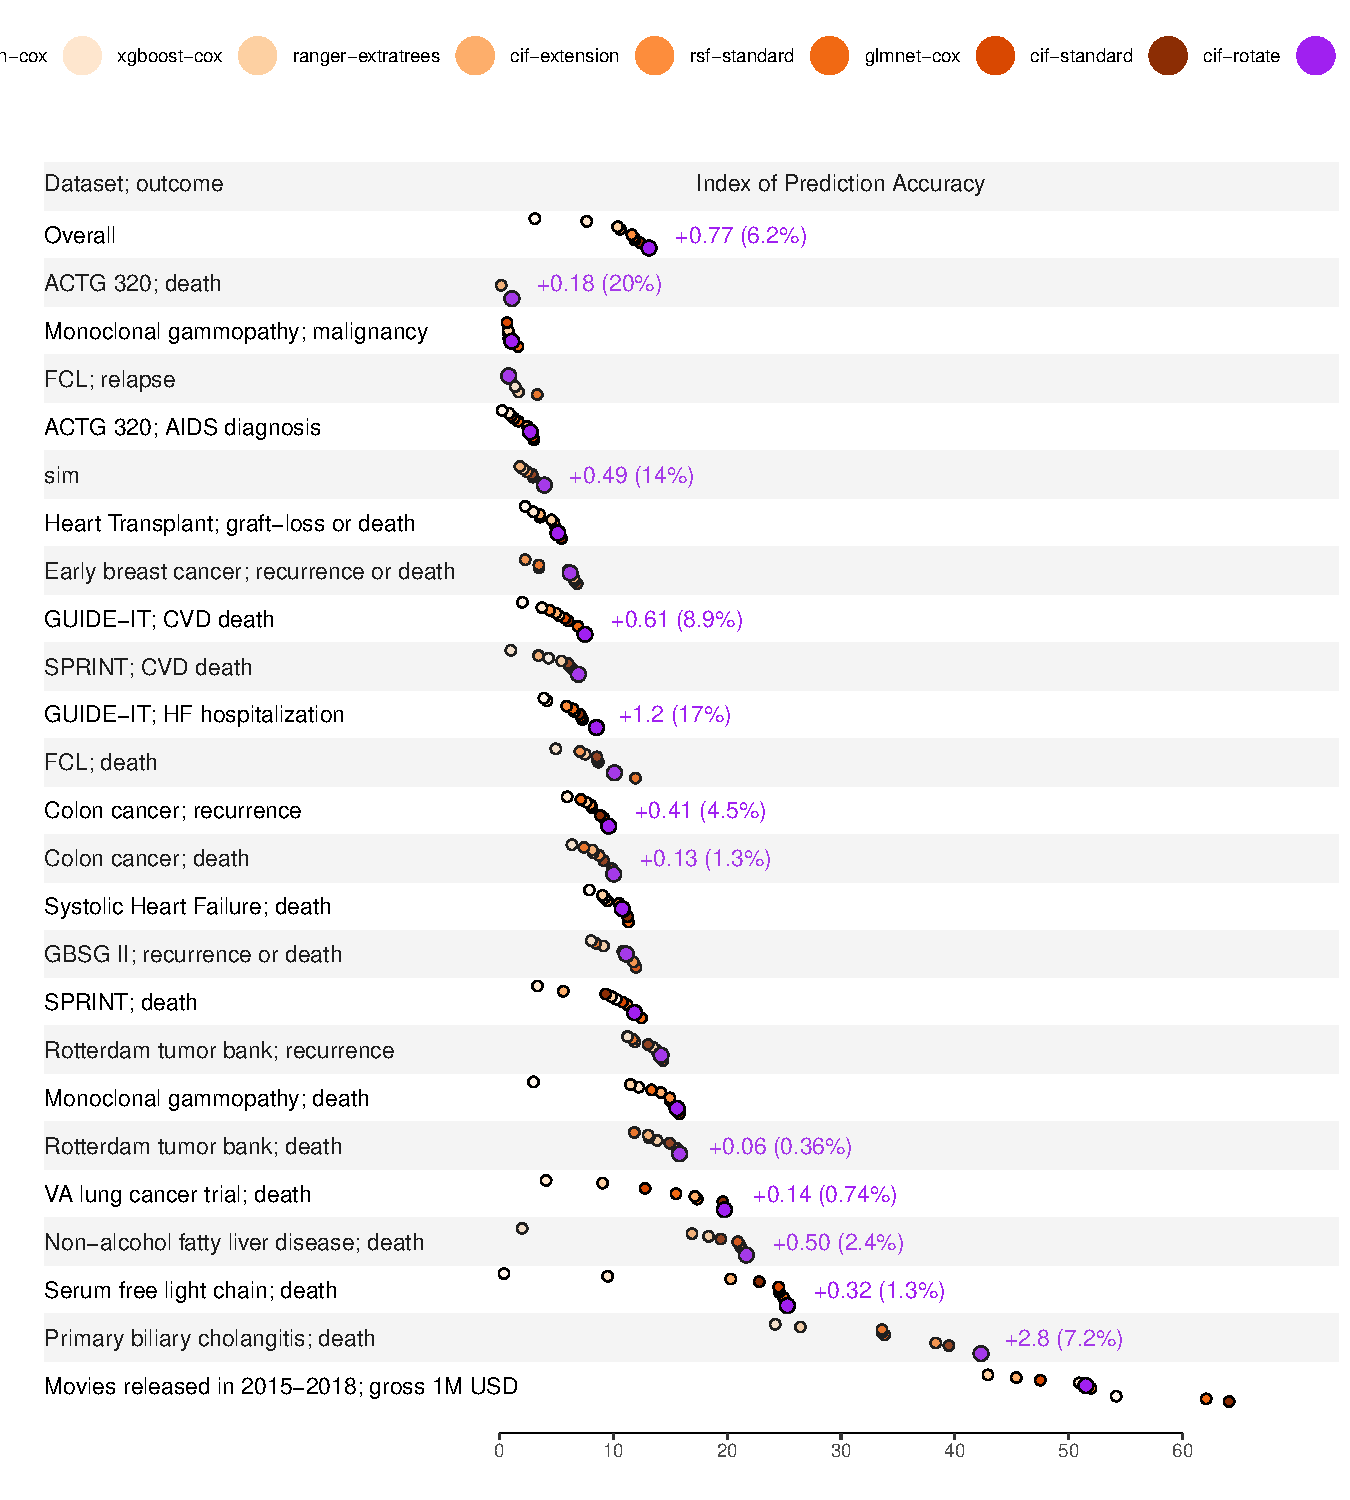
\includegraphics[width=\maxwidth]{figure/unnamed-chunk-2-1} 
\end{knitrout}


\begin{knitrout}
\definecolor{shadecolor}{rgb}{0.969, 0.969, 0.969}\color{fgcolor}
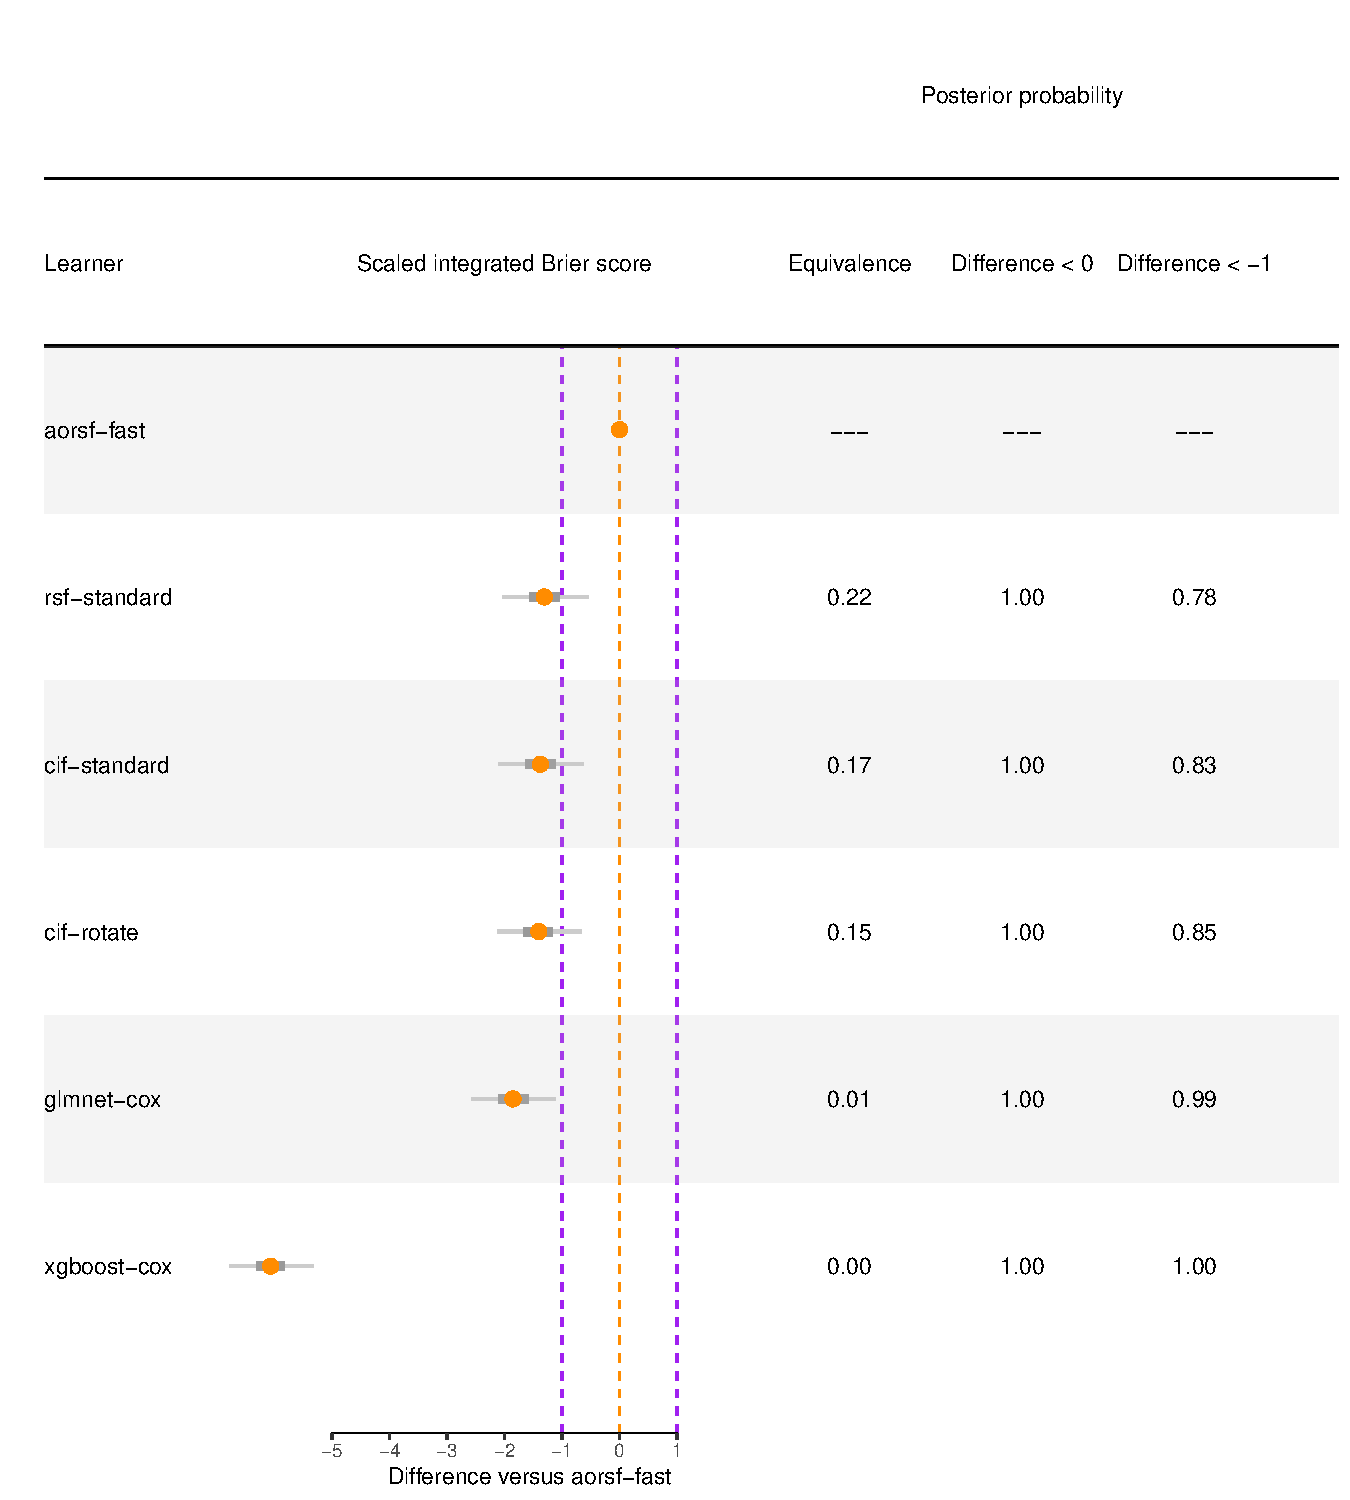
\includegraphics[width=\maxwidth]{figure/unnamed-chunk-3-1} 
\end{knitrout}

\subsection{Benchmark of variable selection}




% Acknowledgements should go at the end, before appendices and references

\acks{Research reported in this publication was supported by the Center for Biomedical Informatics, Wake Forest University School of Medicine}

% Manual newpage inserted to improve layout of sample file - not
% needed in general before appendices/bibliography.

\newpage

\appendix
\section*{Appendix A.}

\begin{knitrout}
\definecolor{shadecolor}{rgb}{0.969, 0.969, 0.969}\color{fgcolor}
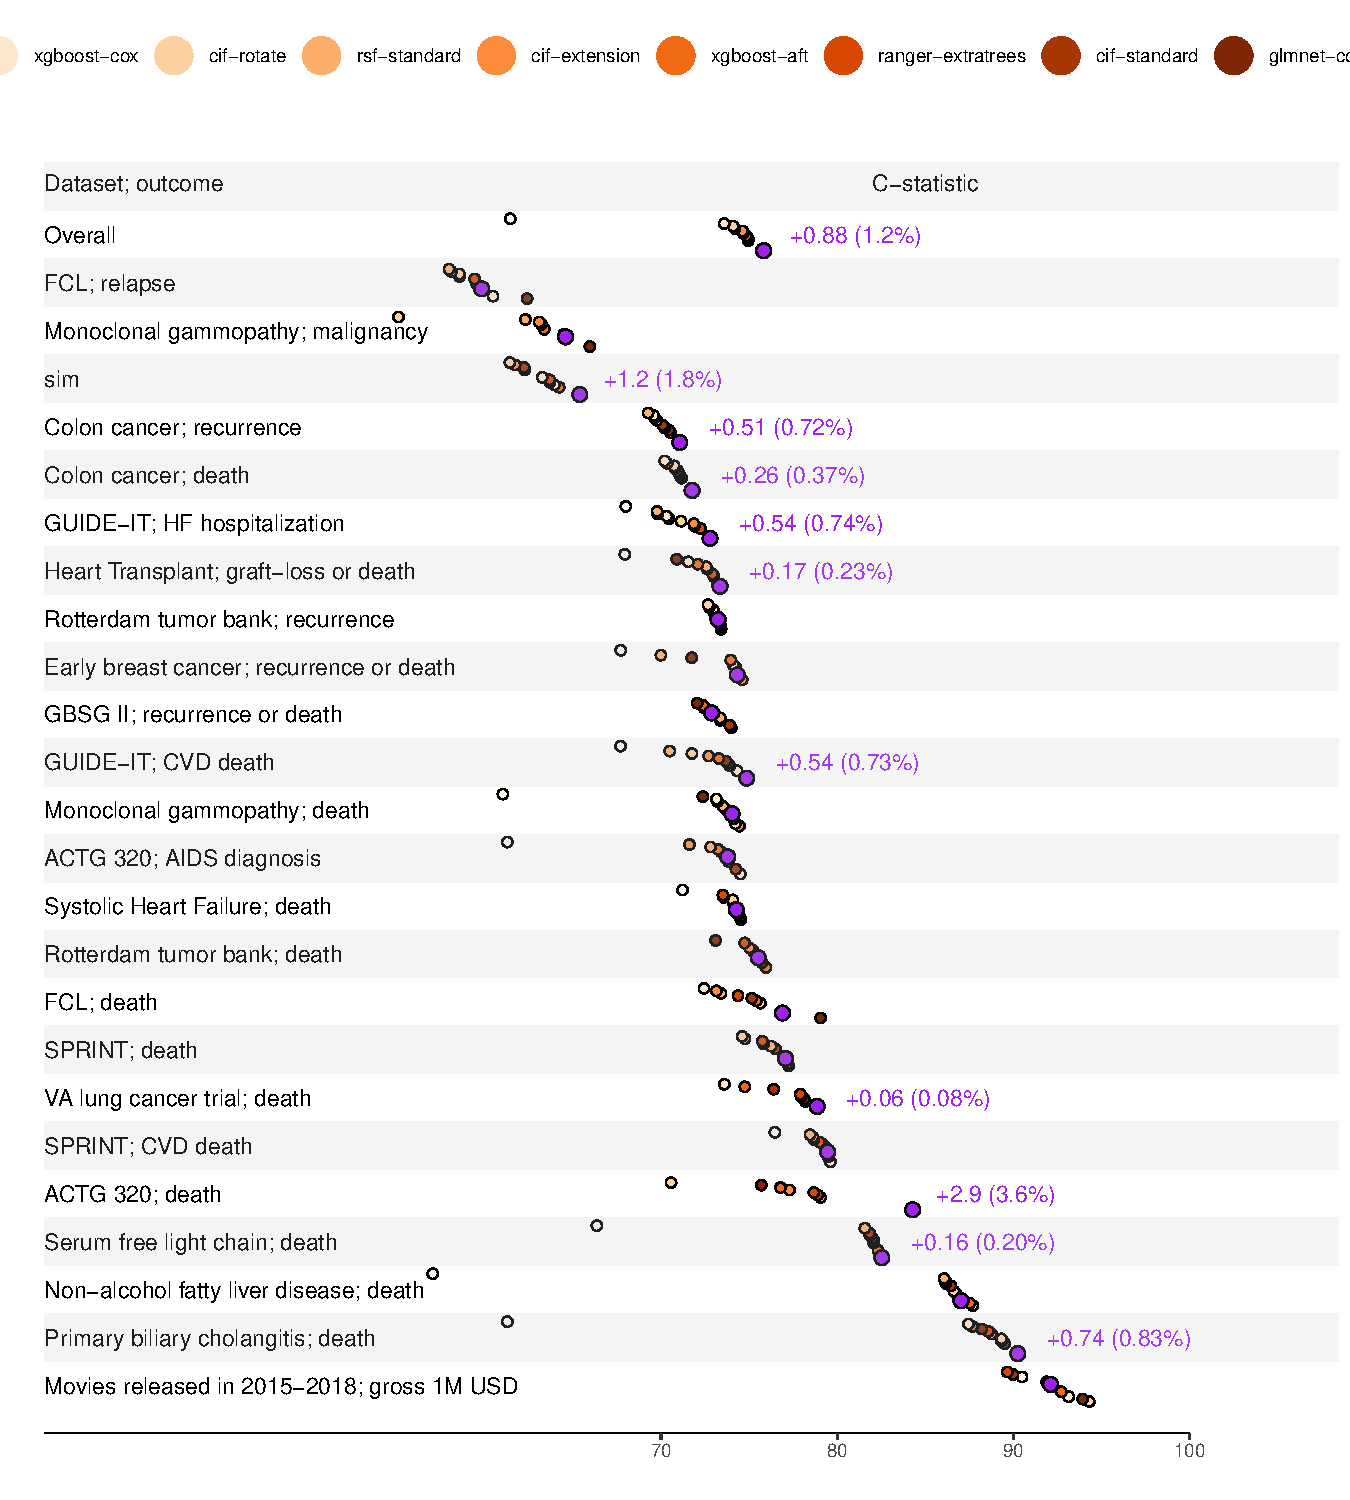
\includegraphics[width=\maxwidth]{figure/unnamed-chunk-4-1} 
\end{knitrout}

\newpage

\begin{knitrout}
\definecolor{shadecolor}{rgb}{0.969, 0.969, 0.969}\color{fgcolor}
\begin{longtable}{lcclccl}
\toprule
\multicolumn{3}{c}{ } & \multicolumn{4}{c}{Computing time, seconds} \\
\cmidrule(l{3pt}r{3pt}){4-7}
\multicolumn{1}{c}{ } & \multicolumn{2}{c}{Performance metric (SD)} & \multicolumn{2}{c}{Fit model} & \multicolumn{2}{c}{Predict risk} \\
\cmidrule(l{3pt}r{3pt}){2-3} \cmidrule(l{3pt}r{3pt}){4-5} \cmidrule(l{3pt}r{3pt}){6-7}
  & Scaled Brier & C-Statistic & Median & Ratio & Median & Ratio\\
\midrule
\endfirsthead
\multicolumn{7}{@{}l}{\textit{(continued)}}\\
\toprule
  & Scaled Brier & C-Statistic & Median & Ratio & Median & Ratio\\
\midrule
\endhead

\endfoot
\bottomrule
\endlastfoot
\addlinespace[0.3em]
\hline
\multicolumn{7}{l}{\textit{\textbf{Overall}}}\\
\hline
\hspace{1em}aorsf-cph(maxit = 15) & 0.136 (0.123) & 0.763 (0.077) & 2.460 & 2.95 & 0.202 & 0.974\\
\hspace{1em}aorsf-cph(maxit = 1) & 0.135 (0.124) & 0.763 (0.077) & 0.833 & 1.00 & 0.207 & 1.00\\
\hspace{1em}aorsf-net & 0.133 (0.127) & 0.762 (0.077) & 53.399 & 64.1 & 0.200 & 0.966\\
\hspace{1em}glmnet-cox & 0.124 (0.136) & 0.753 (0.081) & 0.209 & 0.251 & 0.004 & 0.019\\
\hspace{1em}party-cif & 0.123 (0.111) & 0.755 (0.074) & 1.583 & 1.90 & 4.360 & 21.0\\
\hspace{1em}rfsrc-standard & 0.120 (0.128) & 0.747 (0.080) & 1.554 & 1.86 & 0.150 & 0.725\\
\hspace{1em}obliqueRSF-net & 0.120 (0.093) & 0.762 (0.076) & 268.416 & 322.0 & 18.002 & 86.9\\
\hspace{1em}ranger-extratrees & 0.108 (0.097) & 0.753 (0.073) & 0.217 & 0.261 & 0.211 & 1.02\\
\hspace{1em}aorsf-random & 0.102 (0.092) & 0.740 (0.072) & 1.857 & 2.23 & 0.191 & 0.924\\
\hspace{1em}xgboost-cox & 0.080 (0.114) & 0.740 (0.095) & 3.645 & 4.37 & 0.005 & 0.024\\
\hspace{1em}xgboost-aft & -3.86 (5.01) & 0.753 (0.078) & 12.587 & 15.1 & 0.008 & 0.039\\
\addlinespace[0.3em]
\hline
\multicolumn{7}{l}{\textit{\textbf{ACTG 320; AIDS diagnosis, n = 1151, p = 12}}}\\
\hline
\hspace{1em}aorsf-random & 0.032 (0.017) & 0.749 (0.035) & 1.404 & 2.75 & 0.119 & 1.02\\
\hspace{1em}obliqueRSF-net & 0.031 (0.018) & 0.751 (0.035) & 28.321 & 55.4 & 15.117 & 129.1\\
\hspace{1em}ranger-extratrees & 0.030 (0.014) & 0.739 (0.035) & 0.358 & 0.701 & 0.159 & 1.36\\
\hspace{1em}party-cif & 0.030 (0.024) & 0.749 (0.034) & 1.631 & 3.19 & 4.292 & 36.6\\
\hspace{1em}aorsf-cph(maxit = 15) & 0.029 (0.023) & 0.755 (0.038) & 1.146 & 2.24 & 0.116 & 0.991\\
\hspace{1em}aorsf-cph(maxit = 1) & 0.029 (0.023) & 0.750 (0.040) & 0.511 & 1.00 & 0.117 & 1.00\\
\hspace{1em}aorsf-net & 0.024 (0.027) & 0.750 (0.036) & 19.546 & 38.2 & 0.119 & 1.01\\
\hspace{1em}glmnet-cox & 0.023 (0.026) & 0.755 (0.038) & 0.179 & 0.349 & 0.003 & 0.026\\
\hspace{1em}rfsrc-standard & 0.013 (0.034) & 0.736 (0.037) & 0.638 & 1.25 & 0.060 & 0.514\\
\hspace{1em}xgboost-cox & 0.006 (0.045) & 0.762 (0.035) & 3.745 & 7.33 & 0.003 & 0.026\\
\hspace{1em}xgboost-aft & -8.44 (1.61) & 0.744 (0.034) & 11.231 & 22.0 & 0.006 & 0.051\\
\addlinespace[0.3em]
\hline
\multicolumn{7}{l}{\textit{\textbf{ACTG 320; death, n = 1151, p = 12}}}\\
\hline
\hspace{1em}aorsf-cph(maxit = 15) & 0.013 (0.017) & 0.831 (0.050) & 0.683 & 2.35 & 0.076 & 1.03\\
\hspace{1em}aorsf-cph(maxit = 1) & 0.013 (0.018) & 0.835 (0.050) & 0.291 & 1.00 & 0.074 & 1.00\\
\hspace{1em}aorsf-random & 0.011 (0.013) & 0.802 (0.060) & 1.081 & 3.72 & 0.086 & 1.16\\
\hspace{1em}obliqueRSF-net & 0.010 (0.010) & 0.824 (0.048) & 8.654 & 29.8 & 11.022 & 148.8\\
\hspace{1em}aorsf-net & 0.008 (0.030) & 0.821 (0.054) & 15.008 & 51.6 & 0.085 & 1.14\\
\hspace{1em}ranger-extratrees & 0.005 (0.015) & 0.776 (0.055) & 0.040 & 0.139 & 0.136 & 1.84\\
\hspace{1em}party-cif & 0.001 (0.024) & 0.781 (0.055) & 1.610 & 5.54 & 4.228 & 57.1\\
\hspace{1em}xgboost-cox & -0.003 (0.003) & 0.500 (0.000) & 0.113 & 0.389 & 0.002 & 0.027\\
\hspace{1em}rfsrc-standard & -0.014 (0.048) & 0.785 (0.058) & 0.084 & 0.287 & 0.036 & 0.480\\
\hspace{1em}glmnet-cox & -0.036 (0.073) & 0.735 (0.109) & 0.285 & 0.981 & 0.002 & 0.027\\
\hspace{1em}xgboost-aft & -22.6 (6.75) & 0.774 (0.058) & 10.436 & 35.9 & 0.005 & 0.068\\
\addlinespace[0.3em]
\hline
\multicolumn{7}{l}{\textit{\textbf{Colon cancer; death, n = 929, p = 12}}}\\
\hline
\hspace{1em}aorsf-cph(maxit = 1) & 0.102 (0.016) & 0.720 (0.015) & 0.818 & 1.00 & 0.208 & 1.00\\
\hspace{1em}aorsf-cph(maxit = 15) & 0.101 (0.016) & 0.720 (0.015) & 1.917 & 2.34 & 0.205 & 0.984\\
\hspace{1em}party-cif & 0.100 (0.012) & 0.713 (0.013) & 1.178 & 1.44 & 4.053 & 19.5\\
\hspace{1em}aorsf-random & 0.098 (0.012) & 0.719 (0.015) & 1.640 & 2.00 & 0.191 & 0.918\\
\hspace{1em}aorsf-net & 0.097 (0.016) & 0.720 (0.015) & 51.648 & 63.1 & 0.195 & 0.938\\
\hspace{1em}rfsrc-standard & 0.091 (0.018) & 0.707 (0.013) & 1.462 & 1.79 & 0.149 & 0.716\\
\hspace{1em}obliqueRSF-net & 0.090 (0.007) & 0.720 (0.014) & 241.184 & 294.8 & 44.328 & 213.1\\
\hspace{1em}ranger-extratrees & 0.083 (0.008) & 0.710 (0.015) & 0.571 & 0.698 & 0.251 & 1.21\\
\hspace{1em}glmnet-cox & 0.079 (0.016) & 0.712 (0.020) & 0.110 & 0.135 & 0.004 & 0.019\\
\hspace{1em}xgboost-cox & 0.065 (0.014) & 0.703 (0.015) & 3.225 & 3.94 & 0.004 & 0.019\\
\hspace{1em}xgboost-aft & -1.09 (0.188) & 0.708 (0.013) & 10.975 & 13.4 & 0.006 & 0.029\\
\addlinespace[0.3em]
\hline
\multicolumn{7}{l}{\textit{\textbf{Colon cancer; recurrence, n = 929, p = 12}}}\\
\hline
\hspace{1em}aorsf-cph(maxit = 1) & 0.103 (0.020) & 0.716 (0.019) & 0.819 & 1.00 & 0.210 & 1.00\\
\hspace{1em}aorsf-cph(maxit = 15) & 0.102 (0.019) & 0.715 (0.018) & 1.939 & 2.37 & 0.205 & 0.975\\
\hspace{1em}aorsf-net & 0.099 (0.020) & 0.716 (0.019) & 50.594 & 61.8 & 0.192 & 0.913\\
\hspace{1em}party-cif & 0.096 (0.016) & 0.705 (0.017) & 1.142 & 1.39 & 3.756 & 17.9\\
\hspace{1em}obliqueRSF-net & 0.090 (0.010) & 0.715 (0.018) & 250.487 & 305.8 & 42.658 & 203.0\\
\hspace{1em}aorsf-random & 0.089 (0.014) & 0.705 (0.018) & 1.653 & 2.02 & 0.190 & 0.905\\
\hspace{1em}rfsrc-standard & 0.086 (0.021) & 0.697 (0.017) & 1.473 & 1.80 & 0.151 & 0.719\\
\hspace{1em}ranger-extratrees & 0.080 (0.011) & 0.699 (0.018) & 0.498 & 0.608 & 0.243 & 1.15\\
\hspace{1em}glmnet-cox & 0.078 (0.017) & 0.710 (0.023) & 0.111 & 0.135 & 0.004 & 0.019\\
\hspace{1em}xgboost-cox & 0.061 (0.013) & 0.698 (0.019) & 2.951 & 3.60 & 0.004 & 0.019\\
\hspace{1em}xgboost-aft & -1.16 (0.240) & 0.705 (0.019) & 11.566 & 14.1 & 0.006 & 0.029\\
\addlinespace[0.3em]
\hline
\multicolumn{7}{l}{\textit{\textbf{Early breast cancer; recurrence or death, n = 614, p = 1692}}}\\
\hline
\hspace{1em}obliqueRSF-net & 0.076 (0.024) & 0.754 (0.031) & 1867.133 & 705.0 & 14.418 & 37.5\\
\hspace{1em}aorsf-cph(maxit = 15) & 0.072 (0.027) & 0.752 (0.028) & 5.022 & 1.90 & 0.398 & 1.04\\
\hspace{1em}aorsf-cph(maxit = 1) & 0.070 (0.028) & 0.752 (0.029) & 2.648 & 1.00 & 0.384 & 1.00\\
\hspace{1em}party-cif & 0.069 (0.020) & 0.749 (0.034) & 8.450 & 3.19 & 4.065 & 10.6\\
\hspace{1em}ranger-extratrees & 0.061 (0.022) & 0.742 (0.032) & 0.220 & 0.083 & 0.179 & 0.467\\
\hspace{1em}glmnet-cox & 0.046 (0.031) & 0.724 (0.036) & 5.730 & 2.16 & 0.006 & 0.016\\
\hspace{1em}xgboost-cox & 0.030 (0.028) & 0.745 (0.032) & 2.586 & 0.977 & 0.006 & 0.016\\
\hspace{1em}rfsrc-standard & 0.029 (0.034) & 0.699 (0.030) & 0.606 & 0.229 & 0.617 & 1.61\\
\hspace{1em}aorsf-random & 0.028 (0.015) & 0.692 (0.034) & 3.622 & 1.37 & 0.359 & 0.934\\
\hspace{1em}aorsf-net & 0.025 (0.062) & 0.750 (0.027) & 451.897 & 170.6 & 0.381 & 0.991\\
\hspace{1em}xgboost-aft & -2.92 (0.594) & 0.749 (0.028) & 10.199 & 3.85 & 0.009 & 0.024\\
\addlinespace[0.3em]
\hline
\multicolumn{7}{l}{\textit{\textbf{FCL; death, n = 541, p = 7}}}\\
\hline
\hspace{1em}glmnet-cox & 0.118 (0.034) & 0.790 (0.034) & 0.080 & 0.331 & 0.002 & 0.039\\
\hspace{1em}aorsf-cph(maxit = 15) & 0.098 (0.044) & 0.771 (0.034) & 0.440 & 1.81 & 0.051 & 1.01\\
\hspace{1em}aorsf-cph(maxit = 1) & 0.097 (0.043) & 0.770 (0.034) & 0.243 & 1.00 & 0.051 & 1.00\\
\hspace{1em}aorsf-net & 0.095 (0.044) & 0.762 (0.034) & 13.416 & 55.3 & 0.052 & 1.01\\
\hspace{1em}obliqueRSF-net & 0.089 (0.032) & 0.764 (0.035) & 97.197 & 400.4 & 5.365 & 105.1\\
\hspace{1em}party-cif & 0.083 (0.042) & 0.750 (0.036) & 0.281 & 1.16 & 1.574 & 30.8\\
\hspace{1em}aorsf-random & 0.082 (0.034) & 0.756 (0.032) & 0.459 & 1.89 & 0.052 & 1.02\\
\hspace{1em}ranger-extratrees & 0.072 (0.019) & 0.748 (0.036) & 0.032 & 0.130 & 0.080 & 1.58\\
\hspace{1em}rfsrc-standard & 0.065 (0.053) & 0.736 (0.035) & 0.111 & 0.458 & 0.040 & 0.784\\
\hspace{1em}xgboost-cox & 0.028 (0.055) & 0.694 (0.117) & 0.325 & 1.34 & 0.002 & 0.039\\
\hspace{1em}xgboost-aft & -2.63 (0.596) & 0.757 (0.034) & 7.205 & 29.7 & 0.005 & 0.098\\
\addlinespace[0.3em]
\hline
\multicolumn{7}{l}{\textit{\textbf{FCL; relapse, n = 541, p = 7}}}\\
\hline
\hspace{1em}glmnet-cox & 0.024 (0.020) & 0.611 (0.033) & 0.086 & 0.236 & 0.002 & 0.027\\
\hspace{1em}ranger-extratrees & 0.016 (0.016) & 0.593 (0.024) & 0.031 & 0.086 & 0.081 & 1.07\\
\hspace{1em}obliqueRSF-net & 0.010 (0.018) & 0.589 (0.023) & 221.459 & 610.5 & 10.676 & 141.1\\
\hspace{1em}xgboost-cox & 0.006 (0.016) & 0.591 (0.030) & 1.383 & 3.81 & 0.003 & 0.040\\
\hspace{1em}aorsf-random & 0.006 (0.020) & 0.585 (0.026) & 0.697 & 1.92 & 0.071 & 0.937\\
\hspace{1em}party-cif & 0.003 (0.020) & 0.589 (0.021) & 0.280 & 0.772 & 1.775 & 23.5\\
\hspace{1em}aorsf-cph(maxit = 15) & 0.002 (0.023) & 0.590 (0.027) & 0.709 & 1.95 & 0.075 & 0.997\\
\hspace{1em}aorsf-cph(maxit = 1) & 0.002 (0.023) & 0.589 (0.026) & 0.363 & 1.00 & 0.076 & 1.00\\
\hspace{1em}aorsf-net & 0.001 (0.023) & 0.587 (0.027) & 20.256 & 55.8 & 0.075 & 0.996\\
\hspace{1em}rfsrc-standard & -0.033 (0.031) & 0.572 (0.025) & 0.917 & 2.53 & 0.087 & 1.16\\
\hspace{1em}xgboost-aft & -0.858 (0.311) & 0.578 (0.031) & 6.260 & 17.3 & 0.005 & 0.066\\
\addlinespace[0.3em]
\hline
\multicolumn{7}{l}{\textit{\textbf{GBSG II; recurrence or death, n = 686, p = 10}}}\\
\hline
\hspace{1em}obliqueRSF-net & 0.125 (0.015) & 0.747 (0.018) & 283.036 & 530.9 & 10.993 & 80.3\\
\hspace{1em}party-cif & 0.125 (0.021) & 0.745 (0.020) & 0.465 & 0.873 & 2.516 & 18.4\\
\hspace{1em}aorsf-net & 0.123 (0.024) & 0.741 (0.019) & 37.619 & 70.6 & 0.132 & 0.963\\
\hspace{1em}aorsf-cph(maxit = 15) & 0.121 (0.026) & 0.739 (0.018) & 1.202 & 2.25 & 0.136 & 0.993\\
\hspace{1em}rfsrc-standard & 0.120 (0.026) & 0.739 (0.019) & 1.528 & 2.87 & 0.113 & 0.825\\
\hspace{1em}aorsf-cph(maxit = 1) & 0.117 (0.025) & 0.736 (0.018) & 0.533 & 1.00 & 0.137 & 1.00\\
\hspace{1em}aorsf-random & 0.108 (0.022) & 0.729 (0.025) & 1.226 & 2.30 & 0.130 & 0.948\\
\hspace{1em}ranger-extratrees & 0.094 (0.014) & 0.737 (0.023) & 0.061 & 0.113 & 0.141 & 1.03\\
\hspace{1em}glmnet-cox & 0.088 (0.017) & 0.731 (0.021) & 0.091 & 0.170 & 0.003 & 0.022\\
\hspace{1em}xgboost-cox & 0.086 (0.019) & 0.736 (0.021) & 2.596 & 4.87 & 0.003 & 0.022\\
\hspace{1em}xgboost-aft & -1.10 (0.176) & 0.734 (0.021) & 10.121 & 19.0 & 0.006 & 0.044\\
\addlinespace[0.3em]
\hline
\multicolumn{7}{l}{\textit{\textbf{GUIDE-IT; CVD death, n = 894, p = 59}}}\\
\hline
\hspace{1em}aorsf-cph(maxit = 1) & 0.075 (0.019) & 0.739 (0.030) & 0.578 & 1.00 & 0.130 & 1.00\\
\hspace{1em}aorsf-net & 0.074 (0.020) & 0.738 (0.030) & 27.827 & 48.2 & 0.134 & 1.03\\
\hspace{1em}aorsf-cph(maxit = 15) & 0.072 (0.020) & 0.738 (0.029) & 1.369 & 2.37 & 0.129 & 0.993\\
\hspace{1em}obliqueRSF-net & 0.061 (0.015) & 0.736 (0.029) & 220.667 & 382.1 & 11.349 & 87.2\\
\hspace{1em}party-cif & 0.056 (0.015) & 0.732 (0.030) & 1.431 & 2.48 & 3.202 & 24.6\\
\hspace{1em}glmnet-cox & 0.056 (0.041) & 0.704 (0.097) & 0.497 & 0.860 & 0.002 & 0.015\\
\hspace{1em}ranger-extratrees & 0.052 (0.013) & 0.729 (0.032) & 0.521 & 0.902 & 0.182 & 1.40\\
\hspace{1em}rfsrc-standard & 0.048 (0.026) & 0.704 (0.029) & 0.776 & 1.34 & 0.061 & 0.470\\
\hspace{1em}aorsf-random & 0.034 (0.012) & 0.694 (0.033) & 1.064 & 1.84 & 0.134 & 1.03\\
\hspace{1em}xgboost-cox & 0.021 (0.066) & 0.744 (0.024) & 3.668 & 6.35 & 0.003 & 0.023\\
\hspace{1em}xgboost-aft & -4.95 (0.885) & 0.729 (0.027) & 11.776 & 20.4 & 0.007 & 0.054\\
\addlinespace[0.3em]
\hline
\multicolumn{7}{l}{\textit{\textbf{GUIDE-IT; HF hospitalization, n = 894, p = 59}}}\\
\hline
\hspace{1em}aorsf-net & 0.081 (0.019) & 0.719 (0.023) & 54.048 & 60.8 & 0.207 & 1.03\\
\hspace{1em}aorsf-cph(maxit = 15) & 0.081 (0.019) & 0.719 (0.023) & 2.465 & 2.77 & 0.198 & 0.986\\
\hspace{1em}aorsf-cph(maxit = 1) & 0.080 (0.020) & 0.719 (0.024) & 0.889 & 1.00 & 0.200 & 1.00\\
\hspace{1em}ranger-extratrees & 0.073 (0.012) & 0.717 (0.024) & 0.566 & 0.636 & 0.202 & 1.01\\
\hspace{1em}obliqueRSF-net & 0.073 (0.012) & 0.715 (0.025) & 382.769 & 430.5 & 13.800 & 68.9\\
\hspace{1em}party-cif & 0.070 (0.012) & 0.711 (0.024) & 1.381 & 1.55 & 3.363 & 16.8\\
\hspace{1em}rfsrc-standard & 0.059 (0.019) & 0.691 (0.023) & 1.511 & 1.70 & 0.118 & 0.591\\
\hspace{1em}glmnet-cox & 0.053 (0.023) & 0.692 (0.030) & 0.433 & 0.488 & 0.003 & 0.015\\
\hspace{1em}aorsf-random & 0.051 (0.011) & 0.682 (0.025) & 2.100 & 2.36 & 0.196 & 0.980\\
\hspace{1em}xgboost-cox & 0.039 (0.019) & 0.694 (0.027) & 2.967 & 3.34 & 0.002 & 0.010\\
\hspace{1em}xgboost-aft & -2.12 (0.324) & 0.696 (0.025) & 12.660 & 14.2 & 0.006 & 0.030\\
\addlinespace[0.3em]
\hline
\multicolumn{7}{l}{\textit{\textbf{Heart Transplant; graft-loss or death, n = 3787, p = 52}}}\\
\hline
\hspace{1em}aorsf-net & 0.051 (0.007) & 0.730 (0.013) & 126.867 & 33.3 & 1.065 & 1.03\\
\hspace{1em}aorsf-cph(maxit = 1) & 0.050 (0.007) & 0.731 (0.014) & 3.809 & 1.00 & 1.034 & 1.00\\
\hspace{1em}aorsf-cph(maxit = 15) & 0.050 (0.007) & 0.730 (0.013) & 10.098 & 2.65 & 1.029 & 0.995\\
\hspace{1em}party-cif & 0.048 (0.006) & 0.731 (0.012) & 10.755 & 2.82 & 39.378 & 38.1\\
\hspace{1em}rfsrc-standard & 0.048 (0.009) & 0.727 (0.012) & 3.702 & 0.972 & 1.115 & 1.08\\
\hspace{1em}obliqueRSF-net & 0.048 (0.006) & 0.729 (0.013) & 365.863 & 96.1 & 161.863 & 156.6\\
\hspace{1em}ranger-extratrees & 0.044 (0.006) & 0.727 (0.013) & 5.396 & 1.42 & 3.471 & 3.36\\
\hspace{1em}glmnet-cox & 0.035 (0.005) & 0.710 (0.017) & 1.362 & 0.358 & 0.010 & 0.010\\
\hspace{1em}xgboost-cox & 0.032 (0.008) & 0.717 (0.015) & 3.871 & 1.02 & 0.016 & 0.016\\
\hspace{1em}aorsf-random & 0.028 (0.004) & 0.691 (0.014) & 6.272 & 1.65 & 1.040 & 1.01\\
\hspace{1em}xgboost-aft & -4.26 (0.534) & 0.726 (0.012) & 12.730 & 3.34 & 0.009 & 0.009\\
\addlinespace[0.3em]
\hline
\multicolumn{7}{l}{\textit{\textbf{Monoclonal gammopathy; death, n = 1384, p = 8}}}\\
\hline
\hspace{1em}aorsf-cph(maxit = 15) & 0.158 (0.017) & 0.743 (0.011) & 3.015 & 2.22 & 0.332 & 1.00\\
\hspace{1em}aorsf-cph(maxit = 1) & 0.157 (0.017) & 0.742 (0.011) & 1.360 & 1.00 & 0.332 & 1.00\\
\hspace{1em}obliqueRSF-net & 0.155 (0.013) & 0.743 (0.011) & 240.551 & 176.9 & 16.910 & 50.9\\
\hspace{1em}aorsf-net & 0.154 (0.017) & 0.741 (0.011) & 90.724 & 66.7 & 0.325 & 0.979\\
\hspace{1em}party-cif & 0.152 (0.016) & 0.739 (0.012) & 1.585 & 1.17 & 6.240 & 18.8\\
\hspace{1em}rfsrc-standard & 0.150 (0.018) & 0.737 (0.011) & 2.484 & 1.83 & 0.192 & 0.579\\
\hspace{1em}aorsf-random & 0.147 (0.014) & 0.736 (0.012) & 2.999 & 2.21 & 0.316 & 0.951\\
\hspace{1em}glmnet-cox & 0.139 (0.022) & 0.728 (0.014) & 0.121 & 0.089 & 0.004 & 0.012\\
\hspace{1em}xgboost-cox & 0.122 (0.014) & 0.734 (0.012) & 3.480 & 2.56 & 0.005 & 0.015\\
\hspace{1em}ranger-extratrees & 0.116 (0.007) & 0.745 (0.012) & 0.063 & 0.046 & 0.202 & 0.607\\
\hspace{1em}xgboost-aft & -0.863 (0.151) & 0.732 (0.013) & 11.184 & 8.23 & 0.006 & 0.018\\
\addlinespace[0.3em]
\hline
\multicolumn{7}{l}{\textit{\textbf{Monoclonal gammopathy; malignancy, n = 1384, p = 8}}}\\
\hline
\hspace{1em}glmnet-cox & 0.015 (0.011) & 0.650 (0.046) & 0.101 & 0.138 & 0.002 & 0.014\\
\hspace{1em}aorsf-cph(maxit = 15) & 0.009 (0.014) & 0.639 (0.031) & 1.456 & 2.00 & 0.141 & 0.995\\
\hspace{1em}aorsf-cph(maxit = 1) & 0.008 (0.014) & 0.636 (0.030) & 0.728 & 1.00 & 0.142 & 1.00\\
\hspace{1em}ranger-extratrees & 0.007 (0.007) & 0.633 (0.030) & 0.058 & 0.080 & 0.162 & 1.14\\
\hspace{1em}aorsf-random & 0.007 (0.014) & 0.628 (0.029) & 1.149 & 1.58 & 0.140 & 0.983\\
\hspace{1em}xgboost-cox & 0.007 (0.014) & 0.644 (0.040) & 1.932 & 2.65 & 0.002 & 0.014\\
\hspace{1em}aorsf-net & 0.006 (0.014) & 0.634 (0.029) & 23.343 & 32.1 & 0.141 & 0.996\\
\hspace{1em}obliqueRSF-net & 0.005 (0.012) & 0.626 (0.032) & 39.064 & 53.6 & 16.273 & 114.6\\
\hspace{1em}party-cif & 0.004 (0.013) & 0.626 (0.031) & 1.558 & 2.14 & 5.620 & 39.6\\
\hspace{1em}rfsrc-standard & -0.011 (0.018) & 0.611 (0.032) & 0.793 & 1.09 & 0.075 & 0.528\\
\hspace{1em}xgboost-aft & -5.45 (1.09) & 0.630 (0.037) & 9.725 & 13.4 & 0.006 & 0.042\\
\addlinespace[0.3em]
\hline
\multicolumn{7}{l}{\textit{\textbf{Movies released in 2015-2018; gross 1M USD, n = 551, p = 46}}}\\
\hline
\hspace{1em}glmnet-cox & 0.619 (0.029) & 0.941 (0.009) & 0.180 & 0.226 & 0.004 & 0.019\\
\hspace{1em}aorsf-net & 0.531 (0.024) & 0.929 (0.010) & 52.636 & 66.0 & 0.182 & 1.00\\
\hspace{1em}aorsf-cph(maxit = 15) & 0.523 (0.022) & 0.927 (0.010) & 2.814 & 3.53 & 0.182 & 1.00\\
\hspace{1em}rfsrc-standard & 0.521 (0.023) & 0.923 (0.011) & 1.705 & 2.14 & 0.103 & 0.567\\
\hspace{1em}aorsf-cph(maxit = 1) & 0.517 (0.024) & 0.923 (0.011) & 0.797 & 1.00 & 0.181 & 1.00\\
\hspace{1em}xgboost-cox & 0.508 (0.030) & 0.932 (0.010) & 12.812 & 16.1 & 0.006 & 0.033\\
\hspace{1em}party-cif & 0.479 (0.025) & 0.904 (0.015) & 0.393 & 0.493 & 2.302 & 12.7\\
\hspace{1em}ranger-extratrees & 0.432 (0.025) & 0.901 (0.016) & 0.058 & 0.073 & 0.108 & 0.594\\
\hspace{1em}obliqueRSF-net & 0.323 (0.021) & 0.911 (0.015) & 163.647 & 205.2 & 27.707 & 152.7\\
\hspace{1em}aorsf-random & 0.300 (0.025) & 0.850 (0.023) & 1.511 & 1.90 & 0.170 & 0.934\\
\hspace{1em}xgboost-aft & -0.483 (0.078) & 0.927 (0.011) & 50.372 & 63.2 & 0.009 & 0.047\\
\addlinespace[0.3em]
\hline
\multicolumn{7}{l}{\textit{\textbf{Non-alcohol fatty liver disease; death, n = 17549, p = 24}}}\\
\hline
\hspace{1em}aorsf-cph(maxit = 15) & 0.217 (0.010) & 0.868 (0.006) & 50.582 & 2.70 & 43.776 & 1.15\\
\hspace{1em}aorsf-cph(maxit = 1) & 0.217 (0.010) & 0.869 (0.006) & 18.704 & 1.00 & 37.967 & 1.00\\
\hspace{1em}aorsf-net & 0.214 (0.010) & 0.865 (0.006) & 478.494 & 25.6 & 37.231 & 0.981\\
\hspace{1em}obliqueRSF-net & 0.213 (0.010) & 0.868 (0.006) & 1560.671 & 83.4 & 6530.150 & 172.0\\
\hspace{1em}rfsrc-standard & 0.212 (0.011) & 0.860 (0.007) & 12.257 & 0.655 & 1.293 & 0.034\\
\hspace{1em}glmnet-cox & 0.211 (0.011) & 0.860 (0.006) & 1.509 & 0.081 & 0.464 & 0.012\\
\hspace{1em}party-cif & 0.208 (0.009) & 0.863 (0.006) & 72.349 & 3.87 & 716.204 & 18.9\\
\hspace{1em}ranger-extratrees & 0.184 (0.007) & 0.860 (0.006) & 44.210 & 2.36 & 96.730 & 2.55\\
\hspace{1em}aorsf-random & 0.144 (0.006) & 0.838 (0.007) & 25.720 & 1.38 & 37.114 & 0.978\\
\hspace{1em}xgboost-cox & 0.022 (0.015) & 0.876 (0.006) & 9.865 & 0.527 & 1.013 & 0.027\\
\hspace{1em}xgboost-aft & -7.06 (0.796) & 0.874 (0.006) & 29.664 & 1.59 & 1.001 & 0.026\\
\addlinespace[0.3em]
\hline
\multicolumn{7}{l}{\textit{\textbf{Primary biliary cholangitis; death, n = 276, p = 19}}}\\
\hline
\hspace{1em}aorsf-cph(maxit = 1) & 0.418 (0.048) & 0.905 (0.023) & 0.191 & 1.00 & 0.045 & 1.00\\
\hspace{1em}aorsf-cph(maxit = 15) & 0.408 (0.047) & 0.902 (0.023) & 0.443 & 2.32 & 0.047 & 1.05\\
\hspace{1em}aorsf-net & 0.402 (0.044) & 0.901 (0.024) & 14.653 & 76.7 & 0.046 & 1.03\\
\hspace{1em}rfsrc-standard & 0.378 (0.048) & 0.890 (0.026) & 0.101 & 0.527 & 0.038 & 0.854\\
\hspace{1em}obliqueRSF-net & 0.363 (0.037) & 0.903 (0.024) & 109.549 & 573.2 & 1.750 & 39.1\\
\hspace{1em}aorsf-random & 0.345 (0.038) & 0.889 (0.022) & 0.433 & 2.27 & 0.046 & 1.03\\
\hspace{1em}party-cif & 0.344 (0.039) & 0.899 (0.027) & 0.194 & 1.02 & 0.401 & 8.95\\
\hspace{1em}glmnet-cox & 0.337 (0.053) & 0.885 (0.027) & 0.101 & 0.526 & 0.002 & 0.045\\
\hspace{1em}ranger-extratrees & 0.270 (0.034) & 0.890 (0.029) & 0.026 & 0.135 & 0.038 & 0.855\\
\hspace{1em}xgboost-cox & 0.263 (0.095) & 0.879 (0.026) & 4.438 & 23.2 & 0.002 & 0.045\\
\hspace{1em}xgboost-aft & -0.985 (0.345) & 0.881 (0.024) & 9.390 & 49.1 & 0.007 & 0.146\\
\addlinespace[0.3em]
\hline
\multicolumn{7}{l}{\textit{\textbf{Rotterdam tumor bank; death, n = 2982, p = 11}}}\\
\hline
\hspace{1em}aorsf-net & 0.170 (0.014) & 0.764 (0.011) & 156.389 & 51.8 & 1.283 & 0.947\\
\hspace{1em}obliqueRSF-net & 0.167 (0.012) & 0.764 (0.012) & 453.760 & 150.2 & 117.582 & 86.7\\
\hspace{1em}aorsf-cph(maxit = 15) & 0.167 (0.014) & 0.762 (0.011) & 7.285 & 2.41 & 1.353 & 0.998\\
\hspace{1em}aorsf-cph(maxit = 1) & 0.165 (0.015) & 0.760 (0.012) & 3.021 & 1.00 & 1.356 & 1.00\\
\hspace{1em}party-cif & 0.164 (0.012) & 0.762 (0.012) & 4.837 & 1.60 & 28.933 & 21.3\\
\hspace{1em}rfsrc-standard & 0.163 (0.014) & 0.759 (0.011) & 3.315 & 1.10 & 1.024 & 0.755\\
\hspace{1em}aorsf-random & 0.157 (0.012) & 0.755 (0.012) & 5.742 & 1.90 & 1.275 & 0.941\\
\hspace{1em}ranger-extratrees & 0.141 (0.007) & 0.751 (0.011) & 3.462 & 1.15 & 2.475 & 1.83\\
\hspace{1em}xgboost-cox & 0.135 (0.014) & 0.756 (0.012) & 3.849 & 1.27 & 0.020 & 0.015\\
\hspace{1em}glmnet-cox & 0.120 (0.010) & 0.732 (0.011) & 0.211 & 0.070 & 0.025 & 0.018\\
\hspace{1em}xgboost-aft & -1.36 (0.159) & 0.763 (0.011) & 15.373 & 5.09 & 0.009 & 0.007\\
\addlinespace[0.3em]
\hline
\multicolumn{7}{l}{\textit{\textbf{Rotterdam tumor bank; recurrence, n = 2982, p = 11}}}\\
\hline
\hspace{1em}obliqueRSF-net & 0.151 (0.011) & 0.739 (0.010) & 533.082 & 162.9 & 134.838 & 89.5\\
\hspace{1em}aorsf-net & 0.150 (0.013) & 0.738 (0.010) & 170.007 & 52.0 & 1.437 & 0.954\\
\hspace{1em}aorsf-cph(maxit = 15) & 0.148 (0.013) & 0.736 (0.010) & 8.035 & 2.46 & 1.523 & 1.01\\
\hspace{1em}party-cif & 0.147 (0.012) & 0.736 (0.010) & 5.107 & 1.56 & 31.190 & 20.7\\
\hspace{1em}aorsf-cph(maxit = 1) & 0.147 (0.013) & 0.735 (0.010) & 3.272 & 1.00 & 1.506 & 1.00\\
\hspace{1em}aorsf-random & 0.143 (0.010) & 0.733 (0.009) & 6.299 & 1.93 & 1.394 & 0.926\\
\hspace{1em}rfsrc-standard & 0.142 (0.013) & 0.733 (0.010) & 3.258 & 0.996 & 0.925 & 0.614\\
\hspace{1em}ranger-extratrees & 0.137 (0.007) & 0.736 (0.009) & 3.429 & 1.05 & 2.687 & 1.78\\
\hspace{1em}glmnet-cox & 0.119 (0.008) & 0.729 (0.010) & 0.252 & 0.077 & 0.022 & 0.014\\
\hspace{1em}xgboost-cox & 0.115 (0.008) & 0.732 (0.011) & 3.302 & 1.01 & 0.022 & 0.015\\
\hspace{1em}xgboost-aft & -1.06 (0.148) & 0.737 (0.010) & 14.130 & 4.32 & 0.010 & 0.007\\
\addlinespace[0.3em]
\hline
\multicolumn{7}{l}{\textit{\textbf{Serum free light chain; death, n = 7874, p = 10}}}\\
\hline
\hspace{1em}aorsf-cph(maxit = 15) & 0.249 (0.013) & 0.824 (0.008) & 19.646 & 2.34 & 17.424 & 0.761\\
\hspace{1em}aorsf-cph(maxit = 1) & 0.249 (0.014) & 0.824 (0.007) & 8.398 & 1.00 & 22.885 & 1.00\\
\hspace{1em}aorsf-net & 0.249 (0.013) & 0.821 (0.008) & 305.832 & 36.4 & 21.792 & 0.952\\
\hspace{1em}glmnet-cox & 0.248 (0.012) & 0.819 (0.007) & 0.615 & 0.073 & 0.234 & 0.010\\
\hspace{1em}obliqueRSF-net & 0.247 (0.012) & 0.820 (0.008) & 1107.351 & 131.9 & 817.888 & 35.7\\
\hspace{1em}ranger-extratrees & 0.243 (0.010) & 0.819 (0.008) & 15.165 & 1.81 & 15.048 & 0.658\\
\hspace{1em}party-cif & 0.243 (0.012) & 0.817 (0.008) & 19.999 & 2.38 & 155.997 & 6.82\\
\hspace{1em}rfsrc-standard & 0.242 (0.013) & 0.814 (0.008) & 6.781 & 0.807 & 0.620 & 0.027\\
\hspace{1em}aorsf-random & 0.230 (0.012) & 0.815 (0.008) & 14.450 & 1.72 & 20.496 & 0.896\\
\hspace{1em}xgboost-cox & 0.091 (0.035) & 0.822 (0.008) & 6.066 & 0.722 & 0.136 & 0.006\\
\hspace{1em}xgboost-aft & -2.69 (0.251) & 0.822 (0.008) & 18.993 & 2.26 & 0.650 & 0.028\\
\addlinespace[0.3em]
\hline
\multicolumn{7}{l}{\textit{\textbf{SPRINT; CVD death, n = 9361, p = 174}}}\\
\hline
\hspace{1em}glmnet-cox & 0.071 (0.011) & 0.793 (0.014) & 13.662 & 1.13 & 0.027 & 0.006\\
\hspace{1em}aorsf-cph(maxit = 15) & 0.070 (0.007) & 0.795 (0.013) & 36.982 & 3.06 & 4.419 & 0.951\\
\hspace{1em}aorsf-net & 0.069 (0.009) & 0.794 (0.013) & 358.365 & 29.7 & 4.222 & 0.909\\
\hspace{1em}aorsf-cph(maxit = 1) & 0.069 (0.007) & 0.795 (0.013) & 12.084 & 1.00 & 4.645 & 1.00\\
\hspace{1em}obliqueRSF-net & 0.067 (0.006) & 0.796 (0.014) & 1138.135 & 94.2 & 1242.623 & 267.5\\
\hspace{1em}rfsrc-standard & 0.064 (0.008) & 0.786 (0.015) & 5.499 & 0.455 & 1.247 & 0.268\\
\hspace{1em}party-cif & 0.061 (0.005) & 0.796 (0.013) & 49.198 & 4.07 & 194.676 & 41.9\\
\hspace{1em}ranger-extratrees & 0.054 (0.004) & 0.789 (0.014) & 8.810 & 0.729 & 9.762 & 2.10\\
\hspace{1em}aorsf-random & 0.027 (0.002) & 0.745 (0.016) & 16.090 & 1.33 & 4.634 & 0.998\\
\hspace{1em}xgboost-cox & 0.007 (0.019) & 0.797 (0.013) & 7.793 & 0.645 & 0.031 & 0.007\\
\hspace{1em}xgboost-aft & -10.7 (0.853) & 0.794 (0.013) & 23.758 & 1.97 & 0.017 & 0.004\\
\addlinespace[0.3em]
\hline
\multicolumn{7}{l}{\textit{\textbf{SPRINT; death, n = 9361, p = 174}}}\\
\hline
\hspace{1em}glmnet-cox & 0.123 (0.012) & 0.770 (0.010) & 5.748 & 0.327 & 0.072 & 0.005\\
\hspace{1em}aorsf-cph(maxit = 15) & 0.117 (0.009) & 0.770 (0.010) & 55.731 & 3.17 & 13.261 & 0.895\\
\hspace{1em}aorsf-cph(maxit = 1) & 0.116 (0.009) & 0.769 (0.009) & 17.581 & 1.00 & 14.818 & 1.00\\
\hspace{1em}aorsf-net & 0.114 (0.010) & 0.769 (0.010) & 614.727 & 35.0 & 11.692 & 0.789\\
\hspace{1em}obliqueRSF-net & 0.113 (0.007) & 0.767 (0.010) & 3120.498 & 177.5 & 1215.032 & 82.0\\
\hspace{1em}rfsrc-standard & 0.110 (0.009) & 0.762 (0.010) & 8.948 & 0.509 & 0.805 & 0.054\\
\hspace{1em}party-cif & 0.107 (0.007) & 0.764 (0.010) & 51.458 & 2.93 & 222.920 & 15.0\\
\hspace{1em}ranger-extratrees & 0.097 (0.005) & 0.756 (0.010) & 15.249 & 0.867 & 11.477 & 0.774\\
\hspace{1em}aorsf-random & 0.053 (0.003) & 0.719 (0.011) & 23.393 & 1.33 & 15.908 & 1.07\\
\hspace{1em}xgboost-cox & 0.031 (0.022) & 0.772 (0.009) & 9.917 & 0.564 & 0.082 & 0.006\\
\hspace{1em}xgboost-aft & -4.39 (0.355) & 0.772 (0.010) & 24.150 & 1.37 & 0.027 & 0.002\\
\addlinespace[0.3em]
\hline
\multicolumn{7}{l}{\textit{\textbf{Systolic Heart Failure; death, n = 2231, p = 41}}}\\
\hline
\hspace{1em}glmnet-cox & 0.114 (0.012) & 0.747 (0.012) & 0.272 & 0.113 & 0.010 & 0.013\\
\hspace{1em}obliqueRSF-net & 0.114 (0.011) & 0.747 (0.012) & 388.113 & 161.6 & 56.165 & 70.8\\
\hspace{1em}aorsf-net & 0.112 (0.013) & 0.743 (0.012) & 119.347 & 49.7 & 0.813 & 1.02\\
\hspace{1em}aorsf-cph(maxit = 15) & 0.111 (0.013) & 0.744 (0.012) & 6.734 & 2.80 & 0.798 & 1.01\\
\hspace{1em}party-cif & 0.111 (0.010) & 0.745 (0.012) & 4.287 & 1.79 & 18.913 & 23.8\\
\hspace{1em}aorsf-cph(maxit = 1) & 0.110 (0.015) & 0.744 (0.012) & 2.401 & 1.00 & 0.793 & 1.00\\
\hspace{1em}rfsrc-standard & 0.105 (0.012) & 0.735 (0.012) & 2.526 & 1.05 & 0.273 & 0.345\\
\hspace{1em}ranger-extratrees & 0.092 (0.008) & 0.738 (0.013) & 3.196 & 1.33 & 1.399 & 1.76\\
\hspace{1em}xgboost-cox & 0.090 (0.012) & 0.745 (0.011) & 4.108 & 1.71 & 0.010 & 0.013\\
\hspace{1em}aorsf-random & 0.081 (0.006) & 0.731 (0.013) & 4.722 & 1.97 & 0.779 & 0.983\\
\hspace{1em}xgboost-aft & -1.97 (0.226) & 0.741 (0.010) & 13.112 & 5.46 & 0.008 & 0.010\\
\addlinespace[0.3em]
\hline
\multicolumn{7}{l}{\textit{\textbf{VA lung cancer trial; death, n = 137, p = 8}}}\\
\hline
\hspace{1em}aorsf-net & 0.200 (0.049) & 0.792 (0.036) & 10.492 & 91.2 & 0.024 & 1.00\\
\hspace{1em}aorsf-cph(maxit = 1) & 0.199 (0.049) & 0.790 (0.036) & 0.115 & 1.00 & 0.024 & 1.00\\
\hspace{1em}aorsf-cph(maxit = 15) & 0.198 (0.050) & 0.789 (0.037) & 0.225 & 1.95 & 0.024 & 1.00\\
\hspace{1em}rfsrc-standard & 0.176 (0.046) & 0.781 (0.035) & 0.063 & 0.546 & 0.026 & 1.08\\
\hspace{1em}glmnet-cox & 0.161 (0.044) & 0.784 (0.041) & 0.071 & 0.614 & 0.002 & 0.083\\
\hspace{1em}aorsf-random & 0.151 (0.047) & 0.772 (0.044) & 0.295 & 2.56 & 0.023 & 0.958\\
\hspace{1em}party-cif & 0.129 (0.039) & 0.766 (0.036) & 0.098 & 0.855 & 0.121 & 5.04\\
\hspace{1em}obliqueRSF-net & 0.127 (0.035) & 0.791 (0.034) & 60.532 & 525.9 & 0.660 & 27.5\\
\hspace{1em}ranger-extratrees & 0.091 (0.036) & 0.772 (0.038) & 0.020 & 0.175 & 0.026 & 1.09\\
\hspace{1em}xgboost-cox & 0.069 (0.066) & 0.742 (0.055) & 1.400 & 12.2 & 0.002 & 0.083\\
\hspace{1em}xgboost-aft & -0.010 (0.131) & 0.750 (0.044) & 5.934 & 51.5 & 0.005 & 0.208\\*
\end{longtable}

\end{knitrout}


\vskip 0.2in
\bibliography{main}

\end{document}
